\chapter{Block Cipher Cryptanalysis}
\label{chapter:block_cipher_cryptanalysis} 
\section{Cryptosystem}
\begin{defn}
\citep{cryptosystem_definition_book}A cryptosystem is a five-tuple $\mathcal{(P,C,K,E,D)}$ where the following conditions are satisfied:
\begin{enumerate}
\item $\mathcal{P}$ is a finite set of plaintexts;
\item $\mathcal{C}$ is a finite set of ciphertexts;
\item $K$, the keyspace, is a finite set of keys;
\item For each $K \in \mathcal{K}$ there is an encryption rule $e_K \in \mathcal{E}$ and a corresponding decryption rule $d_K \in \mathcal{D}$. Each $e_K:\mathcal{P} \to \mathcal{C}$ and $d_K \in \mathcal{D} : \mathcal{C} \to \mathcal{P}$ are functions such that $d_K(e_K(x)) = x$ for every plaintext $x \in P$.
\end{enumerate}
\end{defn} 
\begin{figure}[h!]
    \centering
    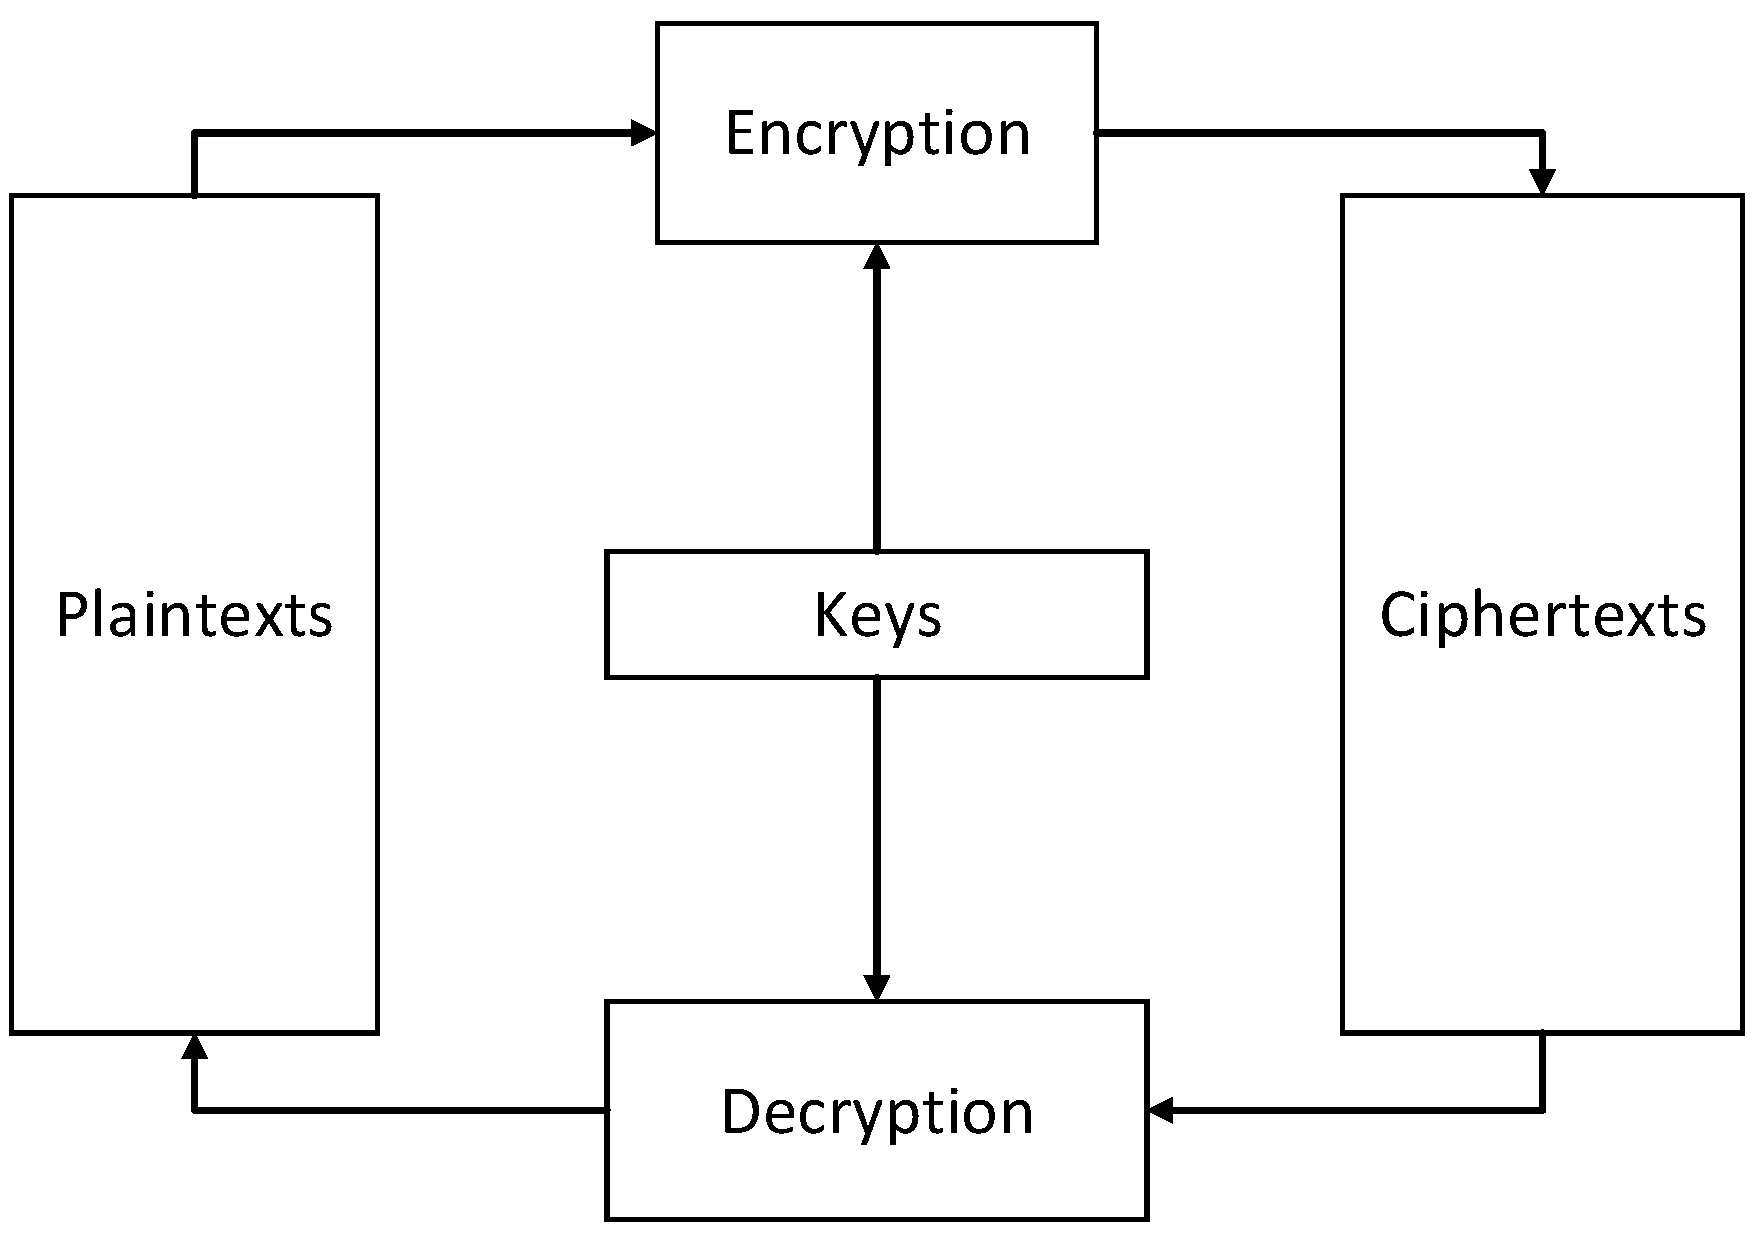
\includegraphics[width=0.7\textwidth , height = 5cm]{images/Cryptosystem}
    \caption{A basic cryptosystem}
    \label{fig:cryptosystem}
\end{figure}That means, a cryptosystem is a set of injective mappings from a finite set of plaintexts to a finite set of ciphertexts. Each key is associated with exactly one mapping. When the plaintext and the ciphertext space are equal the injective mappings are bijective. Figure \ref{fig:cryptosystem} shows a very high level picture of a cryptosystem. However, in this work, the terms \textit{cryptosystem} and \textit{cipher} have been used interchangeably. \par \noindent From the key management point of view, cryptosystems can be classified into two categories. One is public key cryptosystem and the other is symmetric key cryptosystem. In public key cryptosystem, the sender encrypts the message by the receiver\textquotesingle s public key before sending it. The encrypted message can only be decrypted by the receiver\textquotesingle s private key. The security of a public key cryptosystem depends on some computationally hard problems. Among many others, such difficult mathematical problems include discrete logarithm and integer factoring. RSA is a widely known, studied and used public key cryptosystem that uses the hardness of integer factoring as the basis of its security. In a symmetric key cryptosystem, both of the sender and the receiver share the same key which is secret from everyone else. This secret key is used to both encrypt and decrypt the message. Figures \ref{fig:symmetric_key_encryption} and \ref{fig:public_key_encryption} give a very high level view of a symmetric and public key cryptosystem. In both of the figures, Alice is the sender and Bob is the receiver. The security of such symmetric key cryptosystem primarily depends on its randomness, size of ciphertext space and key-length. Block ciphers and stream chiphers are examples of symmetric key cryptosystems. This thesis focuses on block ciphers.
\begin{figure}[h!]
    \centering
    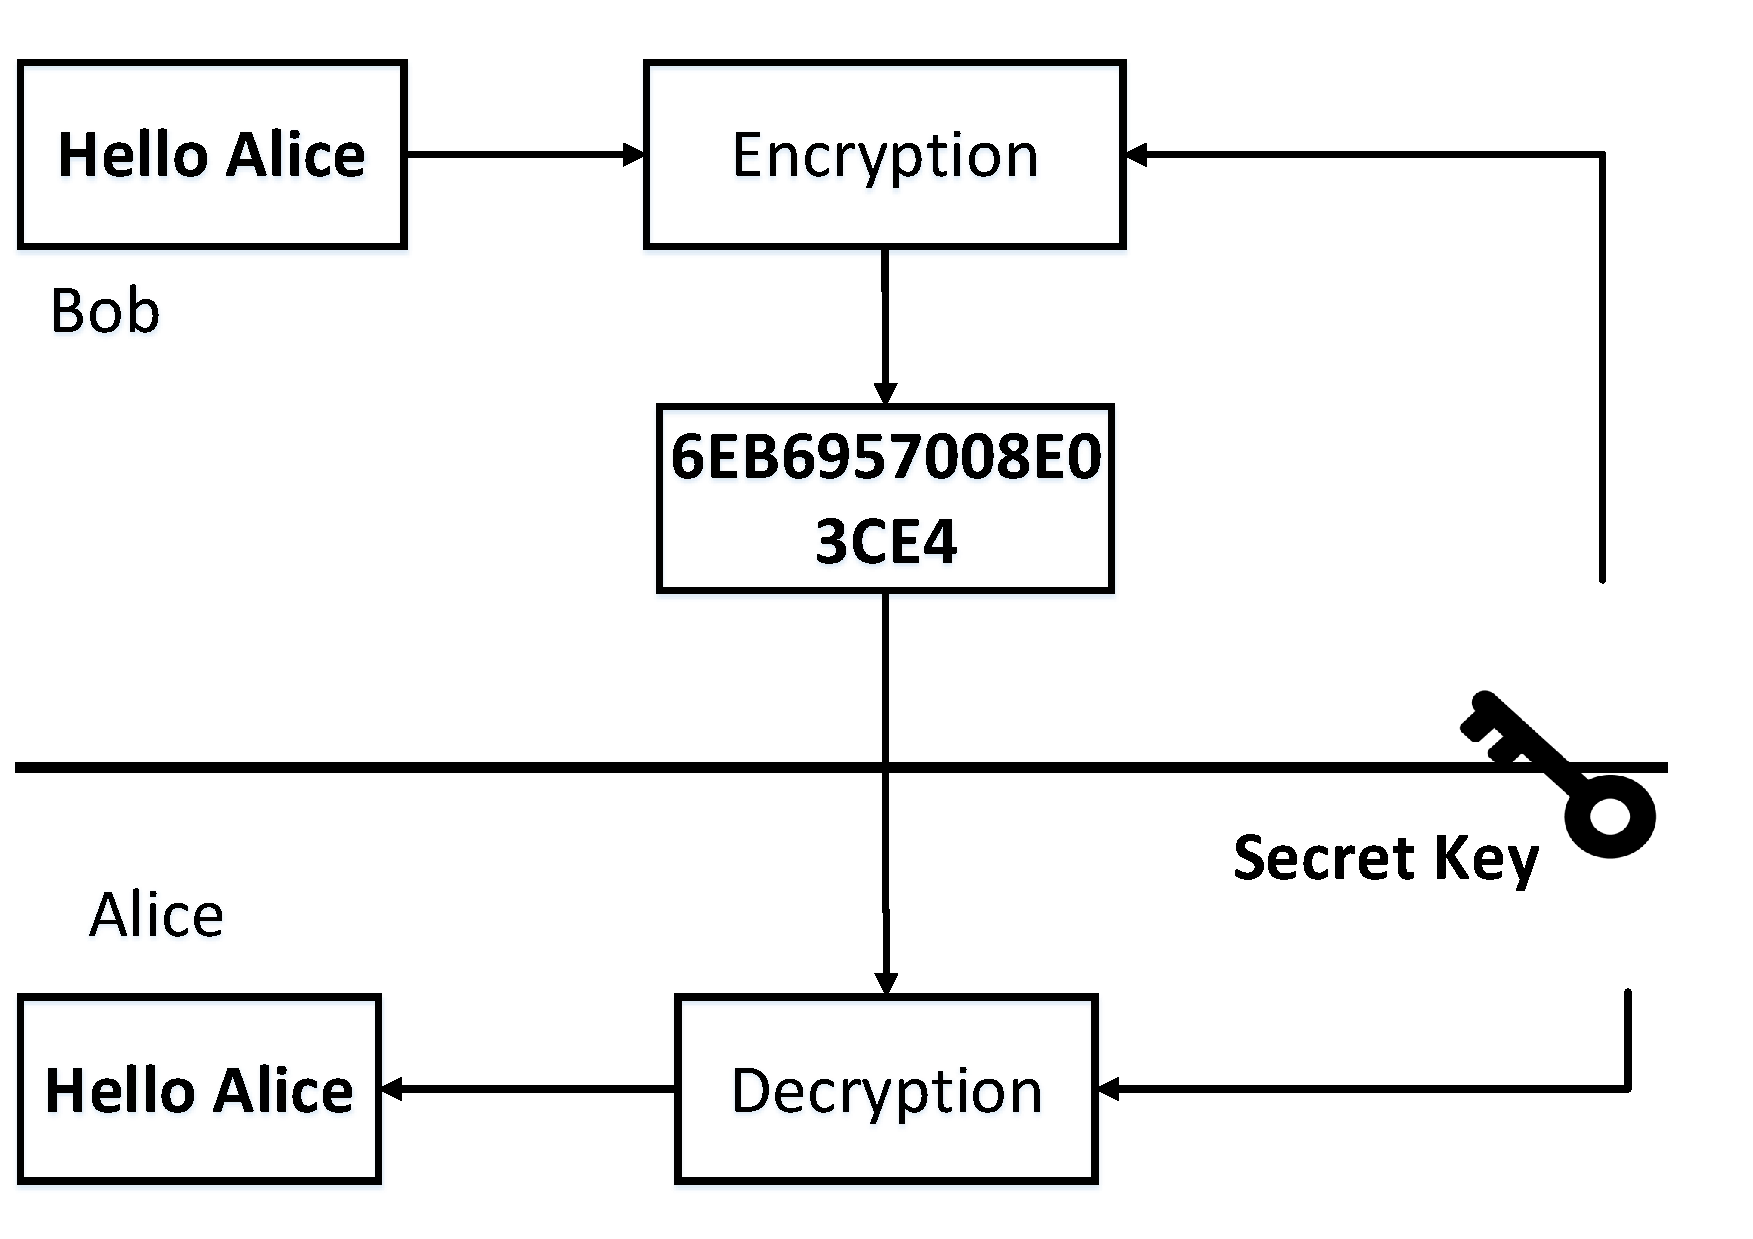
\includegraphics[width=.7\textwidth , height = 6cm]{images/SymmetricKeyEncryption}
    \caption{Symmetric key cryptosystem}
    \label{fig:symmetric_key_encryption}
\end{figure}
\begin{figure}[h!]
    \centering
    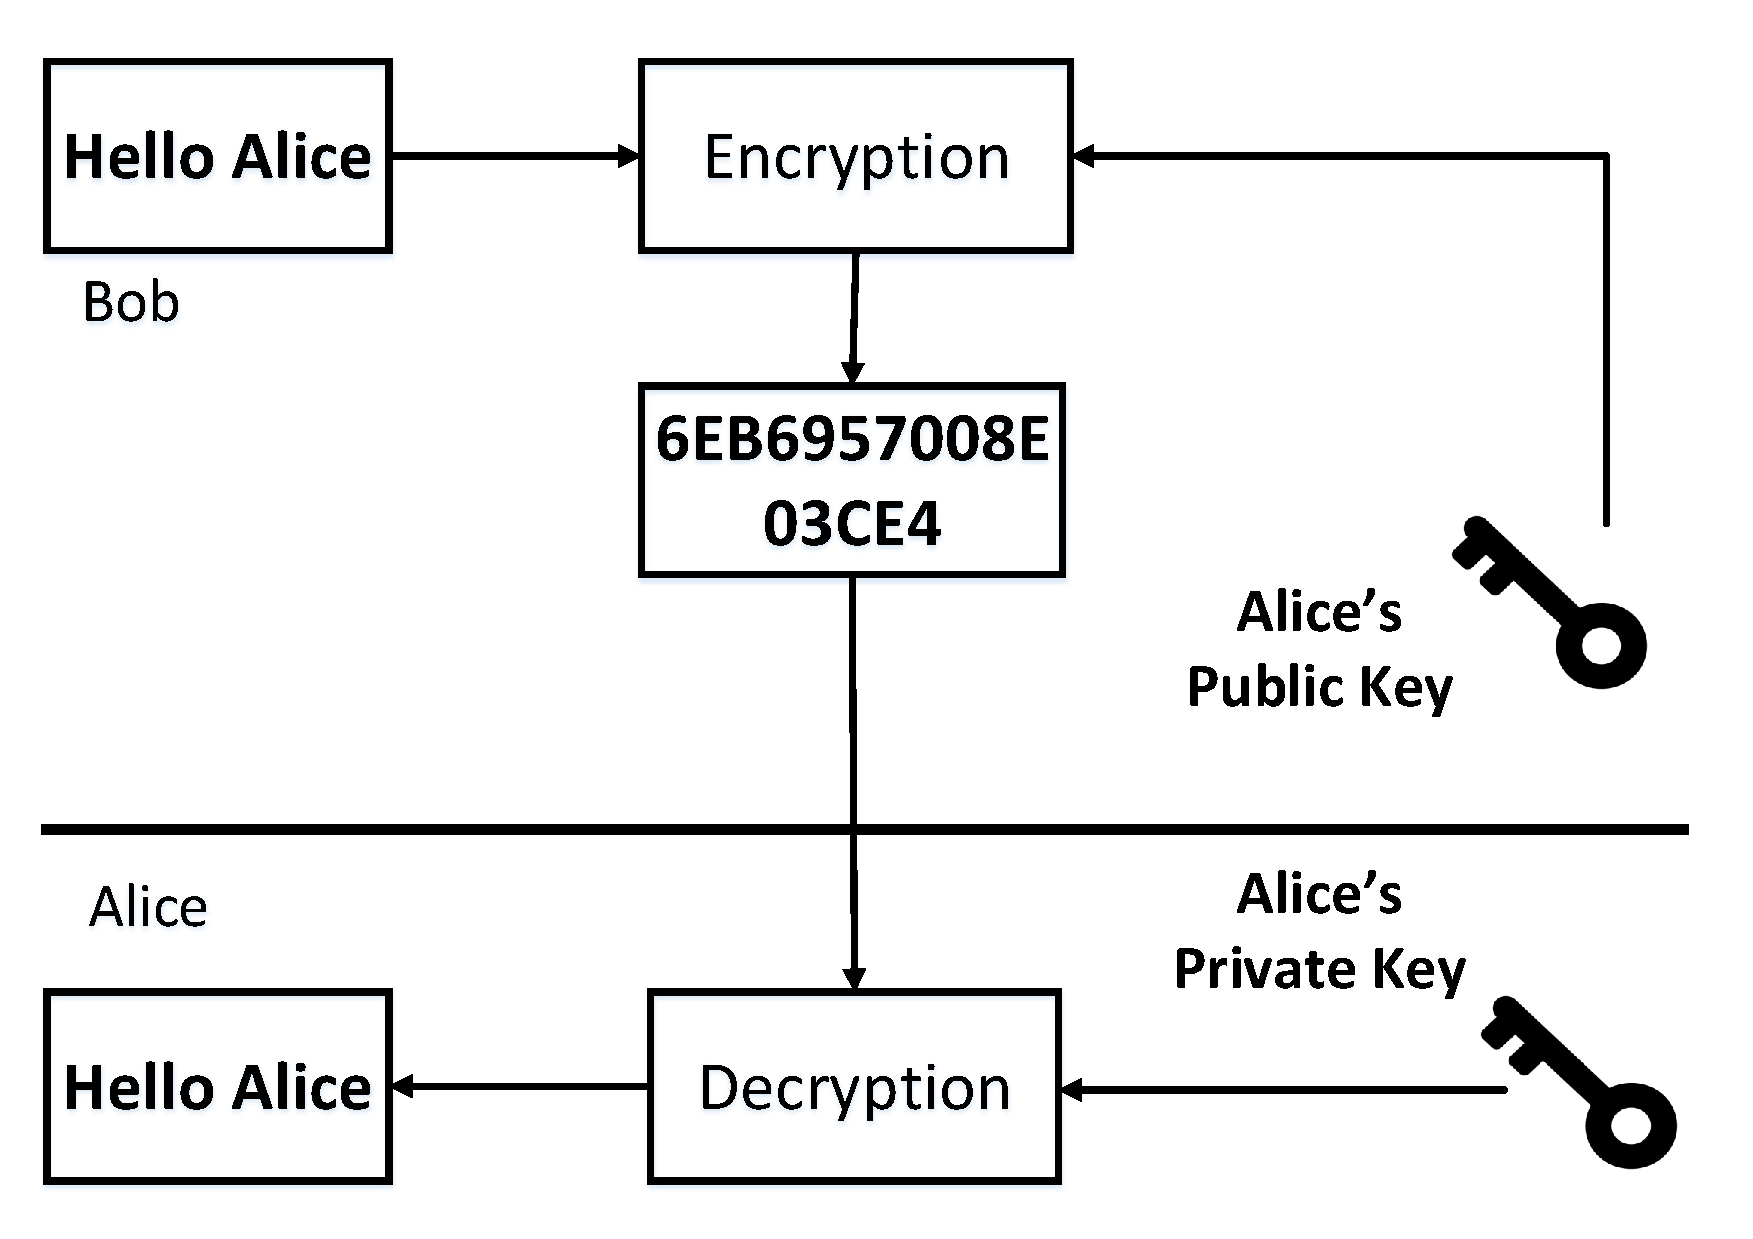
\includegraphics[width=.7\textwidth , height = 6cm]{images/PublicKeyEncryption}
    \caption{Public key cryptosystem}
    \label{fig:public_key_encryption}
\end{figure}
\section{Block Cipher} 
Block cipher is a symmetric key encryption system. The lowest level of granulairty of the encryption system is a block of bits. That is, the data to be encrypted is split into blocks $x_i$ of fixed length $n$ where $i \in \mathbb{N}$. A typical value of $n$ is $128$. And then it encrypts the whole block as a single plaintext and produce the ciphertext of the same length as the plaintext. Generally it can be written as 
\begin{eqnarray*}
\mathcal{P} &=& \mathcal{C} = \mathbb{Z}_2^n \\
\mathcal{K} &=& \mathbb{Z}_2^l
\end{eqnarray*}
For every $k \in \mathcal{K}$ there exists a bijective mapping $E_k:\mathcal{P} \rightarrow \mathcal{C}$. Generally, the mapping $E_k$ consists of repetitive applications of same set of operations. Each repetition is called a round. In each round the cipher often uses a different key which is called the round key. If a block cipher has $r$ number of rounds then there will be $r$ number of round keys denoted by $k^{1}, ...,k^{r}$ and the list of these keys, $(k^1,...,k^{r})$ is called the key schedule. The round keys are generated from a master key $k$ by a fixed key generation algorithm. This key generation algorithm is public. The first round of the cipher takes the plaintext as its input. The output of each round is considered as the input of the next round. The output of the final round is the ciphertext.
\begin{figure}[h!]
    \centering
    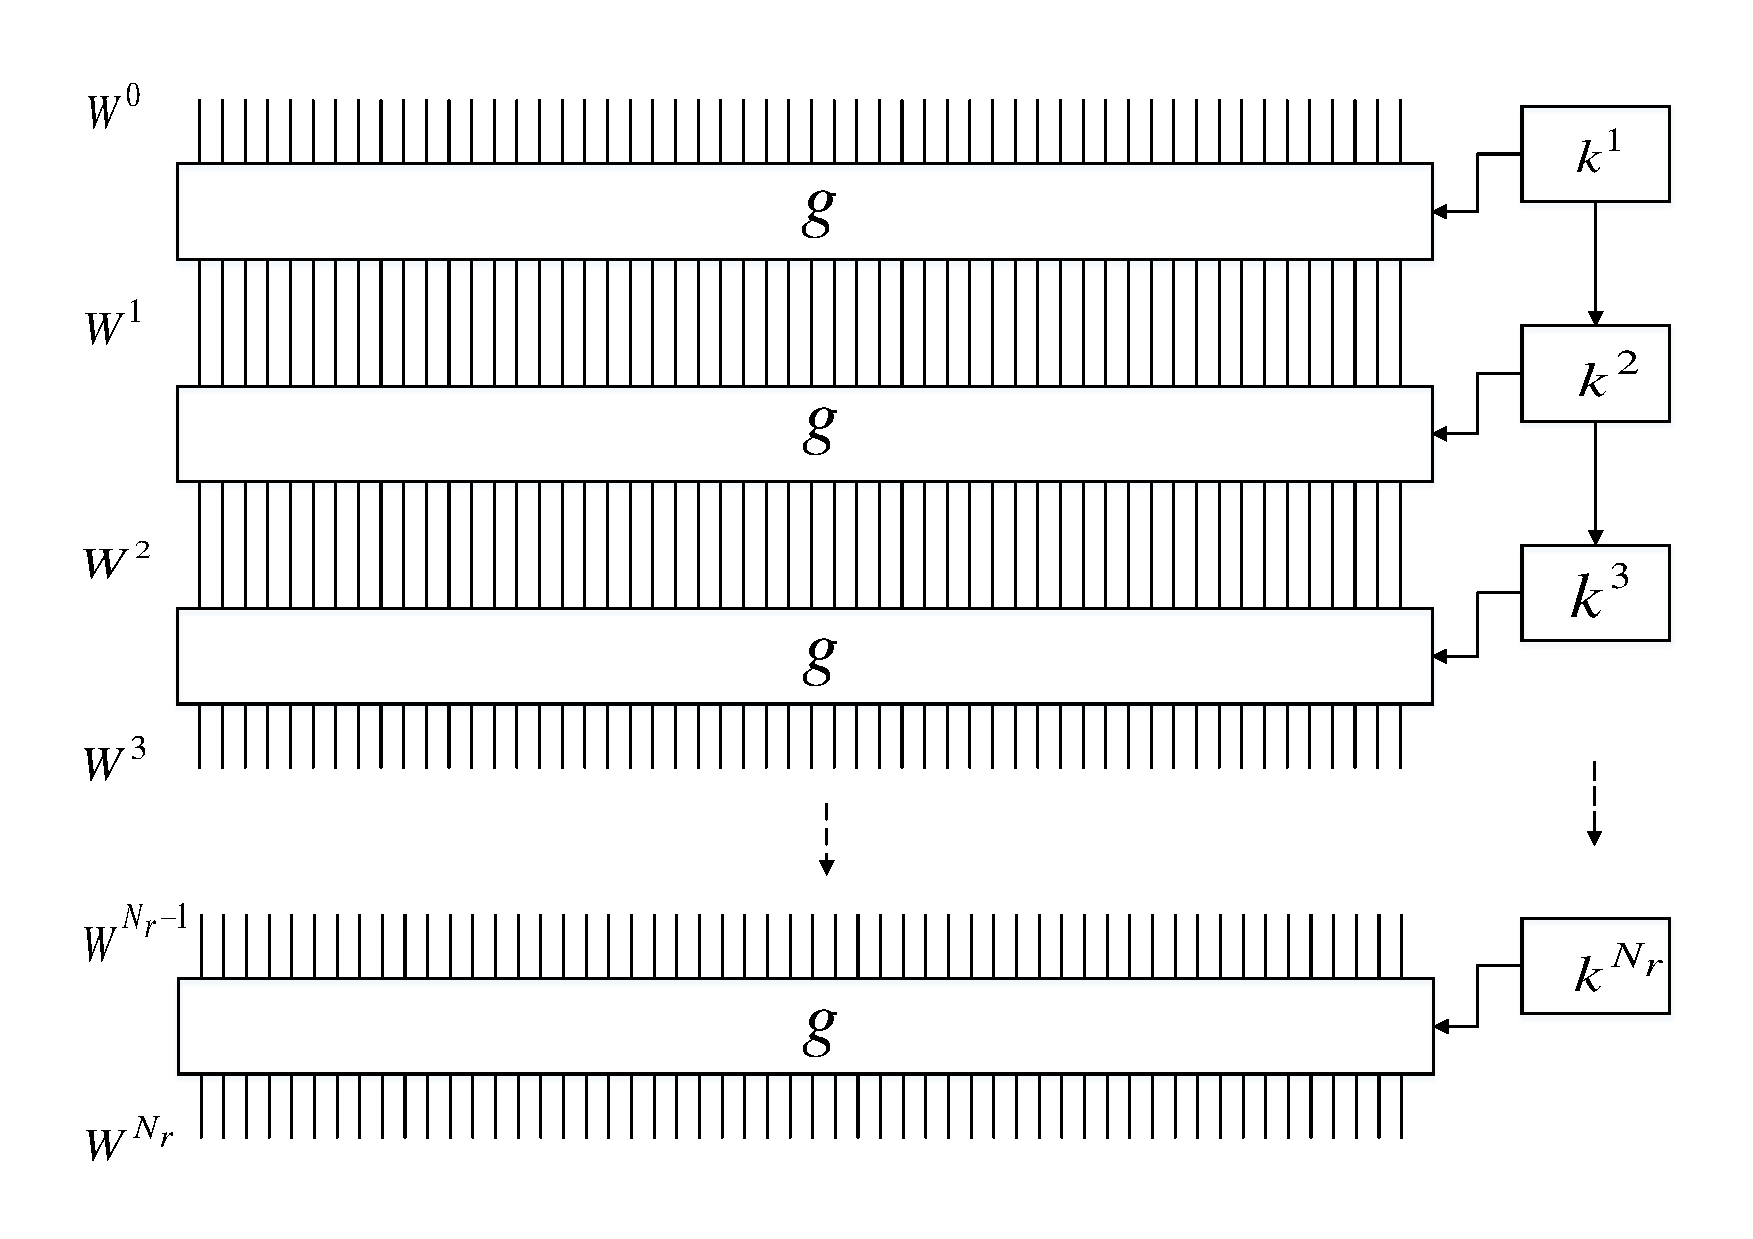
\includegraphics[width=.9\textwidth, height = 7cm]{images/BlockCipher}
    \caption{A block cipher}
    \label{fig:block_cipher}
\end{figure}If we denote the plaintext $x$ by $W^0$ and the ciphertext $E_k(x) = y$ by $W^{r}$ and the round function as $g:\mathcal{P \times \mathcal{K}} \rightarrow \mathcal{C}$, then the encryption of a block cipher can be computed by the Algorithm \ref{Algorithm_block_cipher_encryption}. Figure \ref{fig:block_cipher} shows the operation pictorially.
\begin{algorithm}
\caption{: $E(x,(k^1,...,k^{r}))$}
\label{Algorithm_block_cipher_encryption}
\begin{algorithmic}
\State $W^0 \leftarrow x$
\For {$i \leftarrow 1 \textbf{ to } r$}
	\State $W^{i} \leftarrow g(W^{i-1},k^{i})$
\EndFor
\State $\textbf{return }W^{r}$
\end{algorithmic}
\end{algorithm}
\par \noindent Decryption is applying the inverse of the function $g$ at every round. As we start from the ciphertext, we have to use the key in the reverse order. That is, we have to calculate $W^{r-1} = g^{-1}(W^{r},k^{r})$. Note that, $g$ has to be an injective mapping, otherwise $g^{-1}$ is not well defined. Using this process, we can decrypt the cipher by the Algorithm \ref{Algorithm_block_cipher_decryption}.
\begin{algorithm}
\caption{: $D(y,(k^1,...,k^{r}))$}
\label{Algorithm_block_cipher_decryption}
\begin{algorithmic}
\State $W^{r} \leftarrow y$
\For {$i \leftarrow r \textbf{ to } 1$}
	\State $W^{i-1} \leftarrow g^{-1}(W^{i},k^{i})$
\EndFor
\State $\textbf{return }W^{0}$
\end{algorithmic}
\end{algorithm}
However, based on the detail of function $g$ and the data structure used to hold the states, there are different kinds of block ciphers. The simplest one among those is SPN (Substitution-Permutation Network). In this thesis, SSA is experimented on an SPN named PRESENT. In the following section SPN is discussed in detail.

\subsection{Substitution-Permutation Networks }
\begin{defn} \label{SPN_definition} \citep{spn_definition_book}
Let $a,m$ and $r$ be positive integers, let $\pi_s:\left\lbrace 0,1 \right\rbrace^{a} \rightarrow \left\lbrace 0,1 \right\rbrace^{a}$ be a substitution, and let $\pi_p: \left\lbrace 1,...,am\right\rbrace \rightarrow \left\lbrace 1,...,am\right\rbrace$ be a permutation. Let $\mathcal{P} = \mathcal{C}=\left\lbrace 0,1 \right\rbrace^{am}$, and let $\mathcal{K} \subseteq (\left\lbrace 0,1 \right\rbrace^{am})^{r+1}$ consist of all possible key schedules that could be derived from an initial key $k$ using the key scheduling algorithm. For a key schedule $(k^1,...,k^{r+1})$, the encryption of plaintext is computed as Algorithm \ref{Algorithm_SPN}
\end{defn}
\begin{algorithm}
\caption{: $SPN(x,\pi_s,\pi_p,(k^1,...,k^{r+1}))$}
\label{Algorithm_SPN}
\begin{algorithmic}
\State $W^0 \leftarrow x$
\For {$r \leftarrow 1 \textbf{ to } r - 1$}
	\State $u^{r} \leftarrow W^{r-1} \oplus k^r$
	\For {$i \leftarrow 1 \textbf{ to m}$}
	\State $v^r_{<i>} \leftarrow \pi_s(u^r_{<i>})$
	\EndFor
	\State $W^r \leftarrow (v^r_{\pi_p(1)},...,v^r_{\pi_p(am)})$
\EndFor
\State $u^{r} \leftarrow W^{r-1} \oplus k^{r}$
\For {$i \leftarrow 1 \textbf{ to m}$}
\State $v^{r}_{<i>} \leftarrow \pi_s(u^{r}_{<i>})$
\EndFor
\State $y \leftarrow v^{r} \oplus k^{r+1}$
\State $\textbf{return }y$
\end{algorithmic}
\end{algorithm}Given an $am$ bit binary string, say $x = (x_1,...,x_{am})$, can be regarded as the concatenation of $m$ number of $a$-bit substrings, which can be denoted by $x_{<1>},...,x_{<m>}$. Thus
\begin{eqnarray*}
x &=& x_{<1>}||\cdots||x_{<m>}
\end{eqnarray*} 
and for $1 \leq i \leq m$, we have that 
\begin{eqnarray*}
x_{<i>} &=& (x_{(i-1)a+1},...,x_{ia})
\end{eqnarray*} The SPN consists of $r$ rounds. In each round (except for the last round, which is slightly different), we perform $m$ substitutions using $\pi_s$, followed by a permutation using $\pi_p$. Prior to each substitution operation, we incorporate the round key bits via a simple XOR operation, this is called round key mixing. In Algorithm \ref{Algorithm_SPN}, $u^r$ is the input to the $S$-boxes in round $r$, and $v^r$ is the output of the $S$-boxes after round $r$. $W^r$ is obtained from $v^r$ by applying the permutation $\pi_P$, and then $u^{r+1}$ is constructed from $W^r$ by XOR-ing with the round key $k^{r+1}$ . In the last round, the permutation $\pi_P$ is not applied. Now, we present an SPN as an example.
\begin{exmp}
\label{SPN_Example} \citep{spn_definition_book} Suppose that $a = m = r = 4$. Let $\pi_S$ and $\pi_P$ be defined by Table \ref{table: substitution_table} and \ref{table: permutation_table} respectively, where the input of $\pi_S$ are written in hexadecimal notation, $(0 \leftrightarrow (0,0,0,0), 1 \leftrightarrow (0,0,0,1),...,9 \leftrightarrow (1,0,0,1), A \leftrightarrow (1,0,1,0),...,F \leftrightarrow (1,1,1,1))$. 
\end{exmp}

\begin{table}
\centering
\begin{tabular}{|l|l|l|l|l|l|l|l|l|l|l|l|l|l|l|l|l|}
\hline
$z$ & $0$ & $1$ & $2$ & $3$ & $4$ & $5$  & $6$ & $7$ & $8$ & $9$ & $A$ & $B$ & $C$ & $D$  & $E$ & $F$ \\
\hline
$\pi_S(z)$ & $E$ & $4$ & $D$ & $1$ & $2$ & $F$ & $B$ & $8$ & $3$ & $A$ & $6$ & $C$ & $5$ & $9$ & $0$ & $7$  \\
\hline
\end{tabular}
\caption{Substitution function $\pi_S:\left\lbrace 0,1 \right\rbrace^{4} \rightarrow \left\lbrace 0,1 \right\rbrace^{4}$}
\label{table: substitution_table}
\end{table} 
\begin{table}
\centering
\begin{tabular}{|l|l|l|l|l|l|l|l|l|l|l|l|l|l|l|l|l|}
\hline
$z$ & $0$ & $1$ & $2$ & $3$ & $4$ & $5$  & $6$ & $7$ & $8$ & $9$ & $10$ & $11$ & $12$ & $13$  & $14$ & $15$ \\
\hline
$\pi_P(z)$ & $1$ & $5$ & $9$ & $13$ & $2$ & $6$ & $10$ & $14$ & $3$ & $7$ & $11$ & $15$ & $4$ & $8$ & $12$ & $16$  \\
\hline
\end{tabular}
\caption{Permuation function:$\pi_P: \left\lbrace 0,1,...,15\right\rbrace \rightarrow \left\lbrace 0,1,...,15\right\rbrace$}
\label{table: permutation_table}
\end{table}
\begin{figure}[h!]
    \centering
    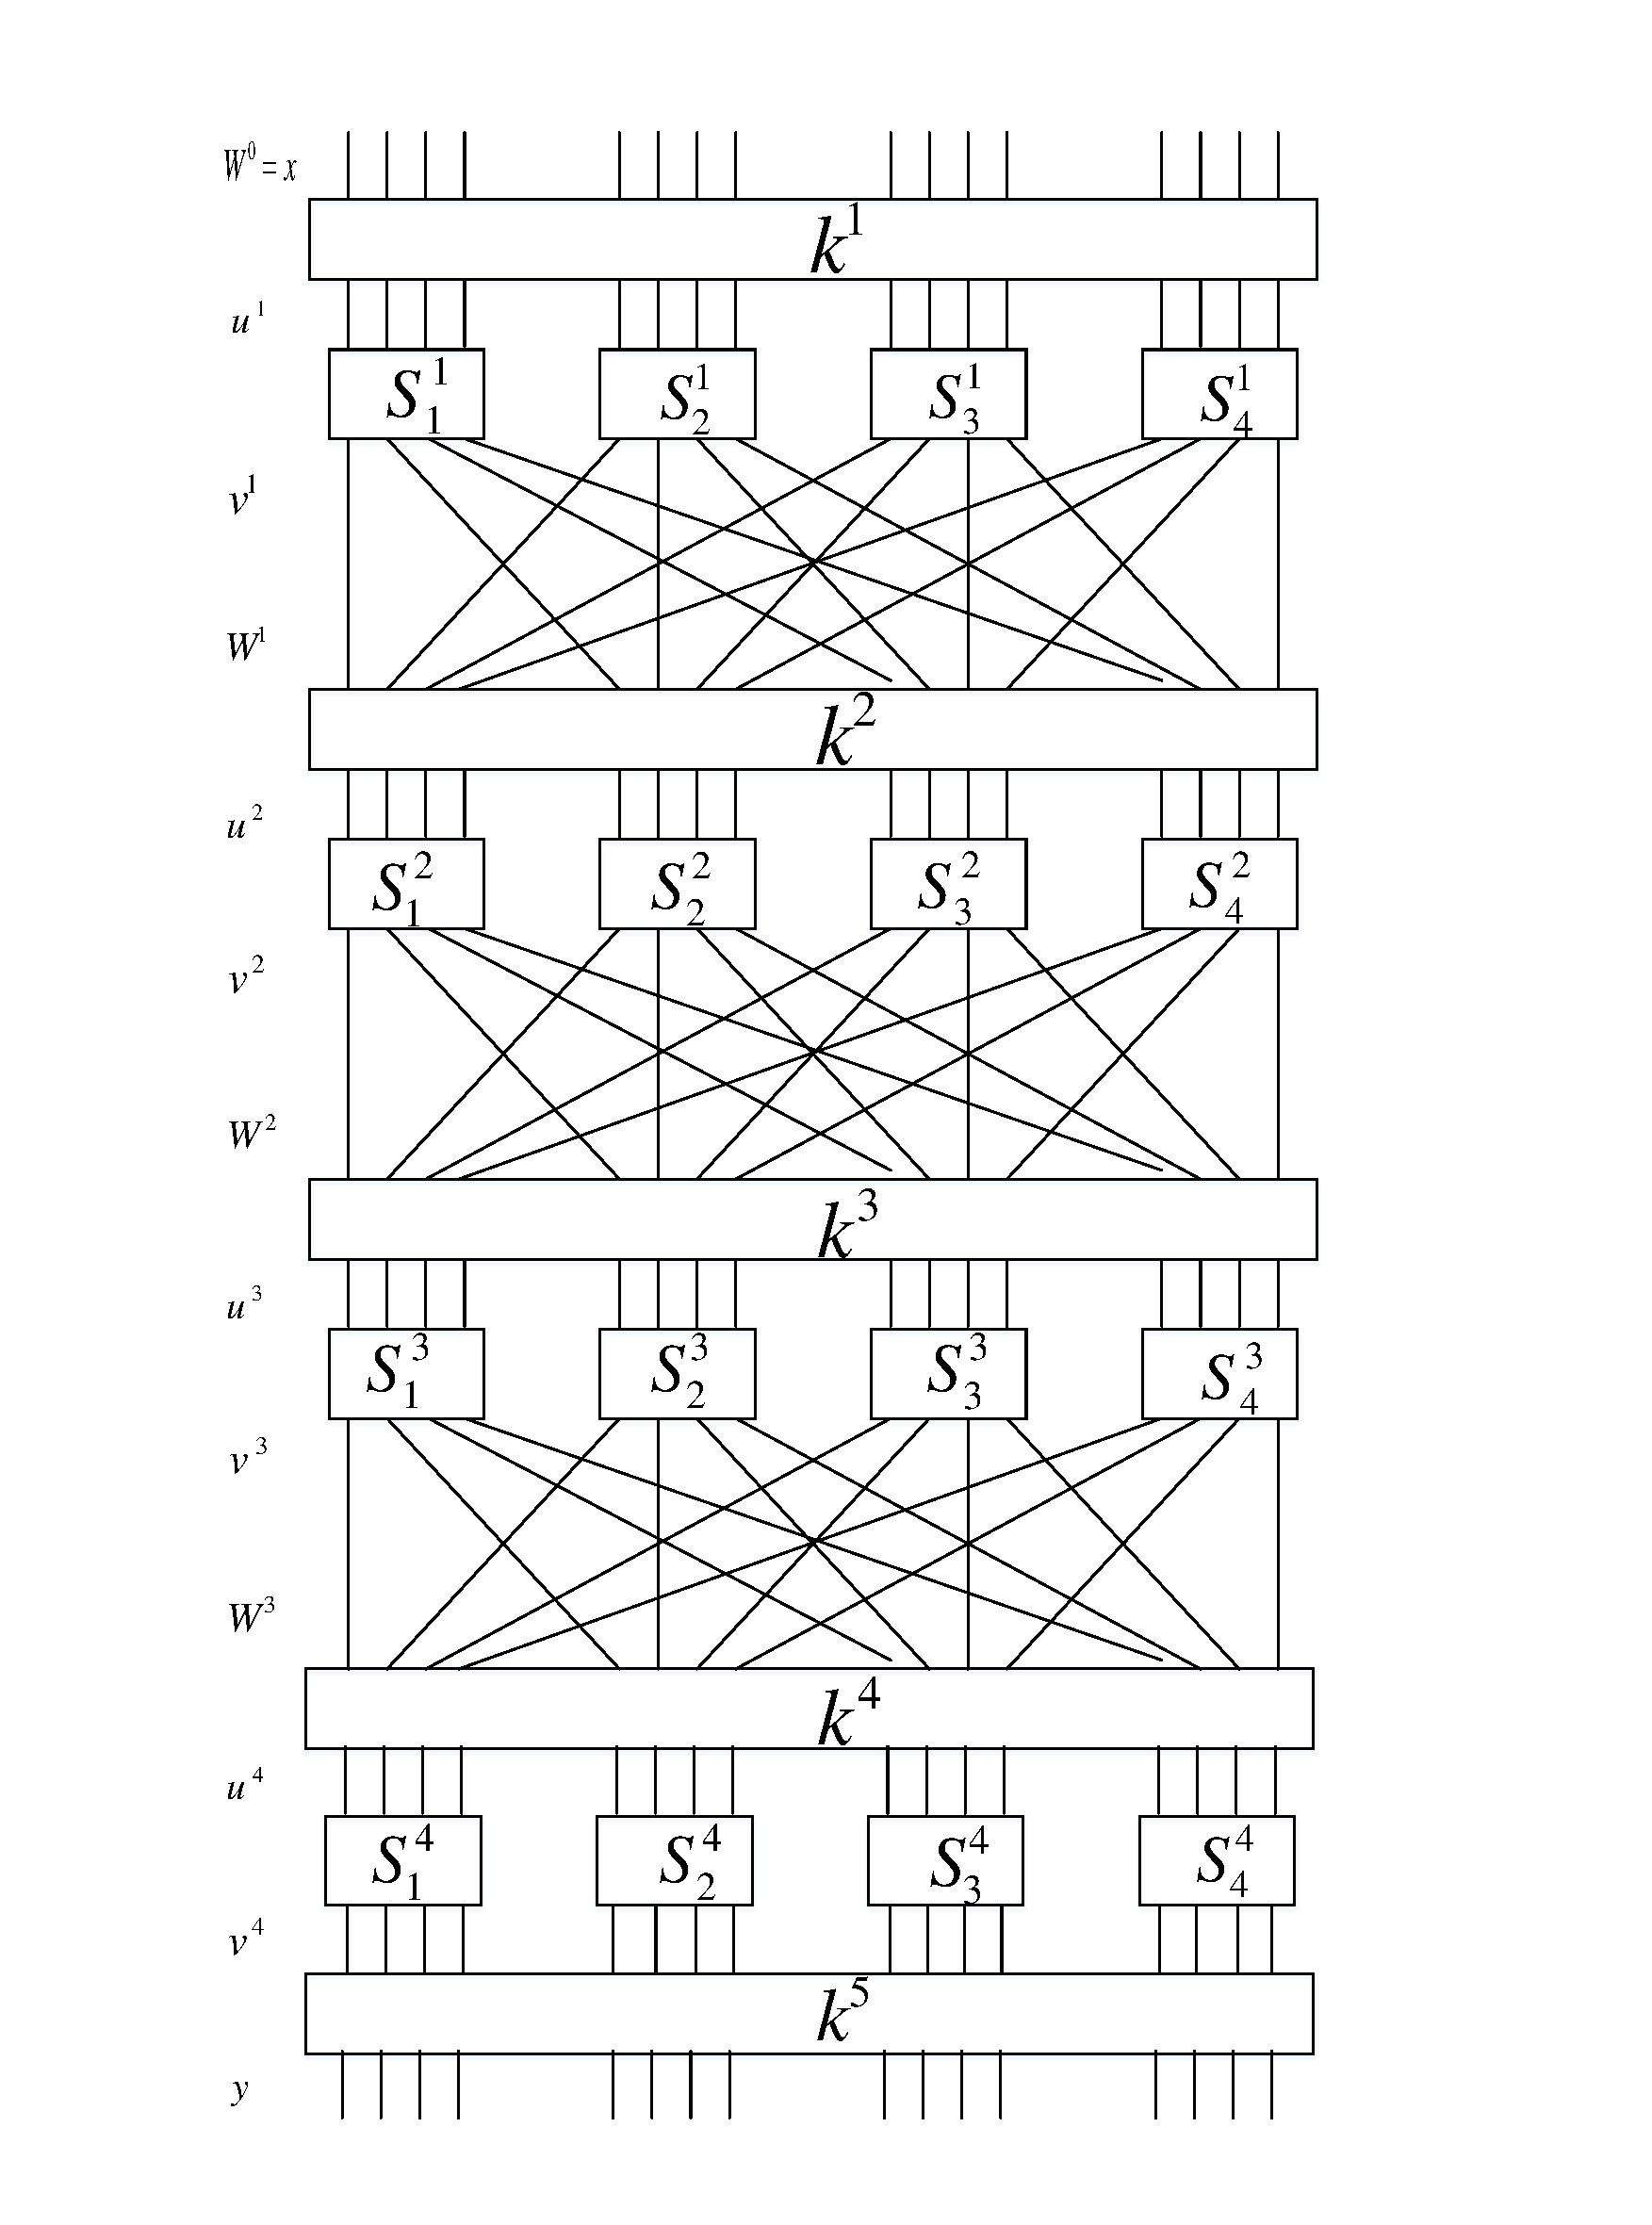
\includegraphics[width=.9\textwidth, height=16cm]{images/SPNDiagram}
    \caption{A substitution-permutation network}
    \label{fig:SPN}
\end{figure}See Figure \ref{fig:SPN} for a pictorial representation of this particular SPN. In this diagram, we have named the $S$-boxes $S_{i}^r$ $(1 \leq i,r \leq 4)$. All $16$ S-boxes incorporate the same substitution function based on $\pi_S$.\par \noindent
In order to complete the description of the SPN, we need to specify a key scheduling algorithm. Here is a simple possibility: suppose that we begin with a $32$-bit key $k = (k_1,...,k_{32}) \in \left\lbrace 0,1 \right\rbrace^{32}$. For $1 \leq r \leq 5$, define $k^r$ to consist of $16$ consecutive bits of $k$, beginning with $k_{4r-3}$. This may not be a very secure way to define a key schedule; we have just chosen something easy for purposes of illustration.\par \noindent SPNs have simple and very efficient design, in both hardware and software. The SPN in Example \ref{SPN_Example} is not secure, if for no other reason that the key length ($32$ bits) is small enough that an exhaustive key search is feasible. However, ``larger" SPNs can be designed that are secure against all known attacks. In this work, we use SPN as the test bed of the statistical model of SSA. As of now, we have defined cryptosystems, block ciphers and SPN. In Section \ref{section:cryptanalysis} we have discussed the general philosophy of statistical cryptnalysis of a block cipher and the state of the art in this field of research. Then we define the SSA formally. In Chapter \ref{chapter:statistical_distinguishers}, we start to derive our statistical model.
\section{Cryptanalysis} \label{section:cryptanalysis}
National Security Agency (NSA) has defined cryptanalysis as the analytic investigation of an information system with the goal of illuminating hidden aspects of that system. It encompasses any systematic analysis aimed at discovering features in, understanding aspects of, or recovering hidden parameters from an information system \cite{def_cryptanalysis}.\par \noindent This thesis work considers the information system to be a block cipher and the systematic analysis exploits the statistical properties of the cipher in question. The process we have followed is broadly known as statistical cryptanalysis. The process includes finding a statistic (preferably parametrized) computable from the cipher system which significantly deviates from the value of the same statistic computed in a uniformly random set up. The process also includes the task of finding the parameter that causes the statistic to deviate the most from random. As the statistic and the parameter is chosen, the cryptanalysis uses a large set of ciphertexts or plaintext-ciphertext pairs associated with the cipher in attack to compute the statistic. Comparing the value of this computed statistic with some known statistic can reveal other hidden information of the cipher. Depending on the statistic used and the way it is exploited, there are many different kinds of statistical cryptanalysis. Some of the very well known statistical cryptanalytic techniques include linear, ML, differential, TD, integral, and SS cryptanalysis. \par \noindent In linear attacks, the statistic used is the correlation of a linear approximation. The linear approximation is obtained by applying a mask on the inputs and a mask on the outputs of the cipher. The correlation of the linear approximation is calculated by comparing how many times the function outputs $1$ and how many times it outputs $0$. Using this statistic, a cipher can be distinguished from random and the last round key can also be partially recovered. Over the years, cryptanalysts have found tricky ways to define this linear approximation. In ML attack, the linear approximation has multiple input and output masks. Based on their correlations, the theoretical distribution of partial plaintext-ciphertext pairs is computed. The input and output masks are chosen in a way so that the distribution deviates by large values from the uniform distribution. \par \noindent On the other hand, in differential attacks, a different statistic is used. It considers the probability of a differential. That is, it checks the probability of pairs of plaintexts with some fixed difference to have certain fixed difference in their corresponding ciphertexts. If a differential is identified for a cipher which has a significantly different probability than in the random case, then that differential can be used to reveal other hidden information of the cipher. In general, the metric used to calculate the difference among the plaintext pairs and ciphertext pairs is bitwise $XOR$. Like linear cryptanalysis, differential cryptanalysis also has its variants. One such variant is truncated differential cryptanalysis. In TD attacks, the differential probability considers only certain bits of plaintexts and ciphertexts while ignoring the other bits. \par \noindent In SSA, the statistic of the distribution of ciphertext or plaintext-ciphertext is considered. Certain bits of the plaintexts are kept fixed while the other bits can vary. SSA encrypts a large number of such plaintexts and exploits the distribution of certain bits of the corresponding ciphertexts. In Section \ref{section:present}, SSA is formally explained  and in Chapter \ref{chapter:statistical_distinguishers}, the derivation of the statistical model of SSA is presented in detail. However, as Collard and Standaert applied this attack on the block cipher PRESENT, we also have selected PRESENT and its small versions \citep{smalpresent} as the test bed of SSA. As a result, before discussing SSA in  detail, it will be useful to discuss the specification of present PRESENT in brief.


\section{PRESENT} \label{section:present}
PRESENT is a Substitution-Permutation Network with a block size of $64$ bits designed by Bogdanov et al. \cite{bogdanov_PRESENT} in $2007$. The recommended key size is $80$ bits, which should be sufficient for the expected applications of the cipher. However, a 128-bit key-schedule is also proposed. The encryption is composed of $31$ rounds. Each of the $31$ rounds consists of a non-linear substitution layer, a linear bitwise permutation layer and a bitwise XOR operation with round key $K_i$ where $1 \leq i \leq 32$. Note that, $K_{32}$ is used for postwhitening. The non-linear layer uses a single $4$-bit S-box which is applied $16$ times in parallel in each round. 
\begin{figure}[h!]
    \centering
    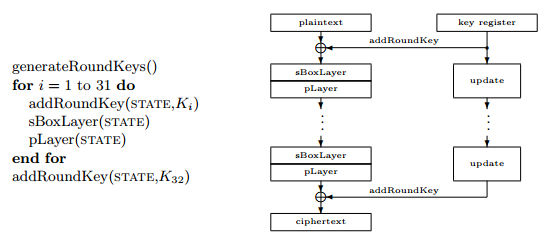
\includegraphics[width=0.9\textwidth]{images/presentCipherAlgorithm}
    \caption{Top-level algorithmic description of PRESENT \cite{SSA_Collard_Standaert}.}
    \label{fig:PRESENT_block_diagram}
\end{figure}  The linear permutation is defined by Table  \ref{table:permutation_table_PRESENT} where bit $i$ of input is moved to bit position $P(i)$. The $4$-bit S-box is defined according to Table 
\ref{table:substitution_table_PRESENT}. We do not mention the key-schedule here as we do not make explicit use of it in our distinguishing attack. Figure $\ref{fig:present_spn}$ shows the substitution-permutation network pictorially for one round.\begin{figure}[h!]
    \centering
    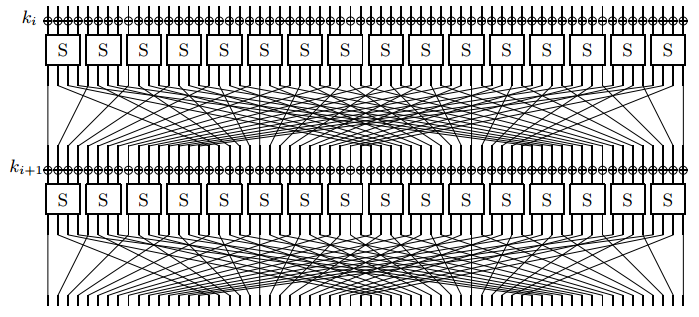
\includegraphics[width=0.9\textwidth]{images/presentCipherSPNetwork}
    \caption{PRESENT SPN \cite{SSA_Collard_Standaert}.}
    \label{fig:present_spn}
\end{figure}
\begin{table}
\centering
\begin{scriptsize}
\begin{tabular}{|l|l|l|l|l|l|l|l|l|l|l|l|l|l|l|l|l|}
\hline
$i$ & $0$ & $1$ & $2$ & $3$ & $4$ & $5$  & $6$ & $7$ & $8$ & $9$ & $10$ & $11$ & $12$ & $13$  & $14$ & $15$ \\
\hline
$p(i)$ & $0$ & $16$ & $32$ & $48$ & $1$ & $17$ & $33$ & $49$ & $2$ & $18$ & $34$ & $50$ & $3$ & $19$ & $35$ & $51$  \\
\hline
\hline
$i$ & $16$ & $17$ & $18$ & $19$ & $20$ & $21$  & $22$ & $23$ & $24$ & $25$ & $26$ & $27$ & $28$ & $29$  & $30$ & $31$ \\
\hline
$p(i)$ & $4$ & $20$ & $36$ & $52$ & $5$ & $21$ & $37$ & $53$ & $6$ & $22$ & $38$ & $54$ & $7$ & $23$ & $39$ & $55$  \\
\hline
\hline
$i$ & $32$ & $33$ & $34$ & $35$ & $36$ & $37$ & $38$ & $39$ & $40$ & $41$ & $42$ & $43$ & $44$ & $45$ & $46$ & $47$ \\
\hline
$p(i)$ & $8$ & $24$ & $40$ & $56$ & $9$ & $25$ & $41$ & $57$ & $10$ & $26$ & $42$ & $58$ & $11$ & $27$ & $43$ & $59$  \\
\hline
\hline
$i$ & $48$ & $49$ & $50$ & $51$ & $52$ & $53$ & $54$ & $55$ & $56$ & $57$ & $58$ & $59$ & $60$ & $61$ & $62$ & $63$ \\
\hline
$p(i)$ & $12$ & $28$ & $44$ & $60$ & $13$ & $29$ & $45$ & $61$ & $14$ & $30$ & $46$ & $62$ & $15$ & $31$ & $37$ & $63$  \\
\hline
\end{tabular}
\end{scriptsize}
\caption{Permutation layer of PRESENT}
\label{table:permutation_table_PRESENT}
\end{table}

\begin{table}
\centering
\begin{scriptsize}
\begin{tabular}{|l|l|l|l|l|l|l|l|l|l|l|l|l|l|l|l|l|}
\hline
$i$ & $0$ & $1$ & $2$ & $3$ & $4$ & $5$  & $6$ & $7$ & $8$ & $9$ & $A$ & $B$ & $C$ & $D$  & $E$ & $F$ \\
\hline
$S[i]$ & $C$ & $5$ & $6$ & $B$ & $9$ & $0$ & $A$ & $D$ & $3$ & $E$ & $F$ & $8$ & $4$ & $7$ & $1$ & $2$  \\
\hline
\end{tabular}
\end{scriptsize}
\caption{S-box of PRESENT (hexadecimal notation).}
\label{table:substitution_table_PRESENT}
\end{table} 


\section{Non-linearity of the S-box in PRESENT}
It is important for any block cipher to be non-linear to be immune against different kind of cryptanalytic attacks \citep{Celine_Kaisa_non_linear_functions,Kaisa_perfect_non_linear_functions}. PRESENT is not an exception. The S-box in PRESENT is a non-linear function. However, being non-linear is not a guarantee for the expected security. Cryptanalysts try to find out linear approximations of the non-linear function with sufficiently deviated correlation which eventually opens up a weakness of the cipher. A good S-box is the one which minimizes deviation of the correlations from zero for all the possible linear approximations. Correlation is a measure of the non-uniformity of a binary function. Let $f:\mathbb{F}_2^n \rightarrow \mathbb{F}_2$ is a boolean function. Then the correlation of function $f$ denoted by $\mathbf{cor}_x\left(f\right)$ is defined in \citep{Celine_Kaisa_Links_2013} as its correlation with the all-zero function as following 
\begin{eqnarray}
\mathbf{cor}_x\left(f\right) &=& \frac{1}{2^n}\left[\# \left\lbrace x \in \mathbb{F}_2^n \;|\;f\left(x\right) = 0 \right\rbrace - \# \left\lbrace x \in \mathbb{F}_2^n \;|\;f\left(x\right) \neq 0 \right\rbrace \right]
\end{eqnarray}
A linear approximation $f:\mathbb{F}_2^n \rightarrow \mathbb{F}_2$ of a vectorial boolean function $\mathbf{F}:\mathbb{F}_2^n \rightarrow \mathbb{F}_2^n$ is developed by considering an input and an output mask $\alpha,\beta \in \mathbb{F}_2^n$ in the following way
\begin{eqnarray}
f_{\left(\alpha,\beta \right)} \left( x \right) &=& \alpha \cdot x \oplus \beta \cdot \mathbf{F}\left( x \right)
\end{eqnarray} where the notation ``$\cdot$'' represents standard inner product.
The S-box used in PRESENT is a vectorial boolean function $S:\mathbb{F}_2^4 \rightarrow \mathbb{F}_2^4$ mentioned in Table \ref{table: substitution_table}. So, given an input mask $\alpha \in \mathbb{F}_2^4$ and an output mask $\beta \in \mathbb{F}_2^4$, and a vectorial boolean function $S$, the correlation of the linear approximation $f_{\left(\alpha,\beta \right)} = \alpha \cdot x \oplus \beta \cdot S\left(x\right)$ is measured as follows:
\begin{eqnarray*}
\mathbf{cor}_x\left(f_{\left(\alpha,\beta \right)}\right) &=& \frac{1}{2^n}\left[\# \left\lbrace x \in \mathbb{F}_2^n \;|\; f_{\left(\alpha,\beta \right)}\left(x\right) = 0 \right\rbrace - \# \left\lbrace x \in \mathbb{F}_2^n\;|\;f_{\left(\alpha,\beta \right)}\left(x\right) \neq 0 \right\rbrace \right]
\end{eqnarray*}
The correlation table of the S-box of PRESENT is given in Table \ref{table:correlation_matrix} \citep{j_y_cho_linear_cryptanalysis}. We have discussed how this table helps in preparing an SSA in Section \ref{section:choosing_ssa_trail}. In Chapter \ref{chapter:experiment}, we have shown in detail how this table helps in finding a feasible SSA attack on SMALLPESENT-$[n]$.
\begin{table}
\centering
\begin{tiny}
\begin{tabular}{|l|l|l|l|l|l|l|l|l|l|l|l|l|l|l|l|}
\hline
$\alpha / \beta$&$1$&$2$&$3$&$4$&$5$&$6$&$7$&$8$&$9$&$A$&$B$&$C$&$D$&$E$&$F$ \\
\hline
$1$&$0$&$\frac{1}{4}$&$0$&$0$&$-\frac{1}{2}$&$0$&$-\frac{1}{2}$&$0$&$0$&$0$&$0$&$0$&$-\frac{1}{2}$&$0$&$\frac{1}{2}$  \\ \hline
$2$&$0$&$\frac{1}{4}$&$\frac{1}{4}$&$-\frac{1}{4}$&$-\frac{1}{4}$&$0$&$0$&$\frac{1}{4}$&$-\frac{1}{4}$&$0$&$\frac{1}{2}$&$0$&$\frac{1}{2}$&$-\frac{1}{4}$&$\frac{1}{4}$  \\ \hline
$3$&$0$&$\frac{1}{4}$&$\frac{1}{4}$&$\frac{1}{4}$&$-\frac{1}{4}$&$-\frac{1}{2}$&$0$&$-\frac{1}{4}$&$\frac{1}{4}$&$-\frac{1}{2}$&$0$&$0$&$0$&$-\frac{1}{4}$&$-\frac{1}{4}$  \\ \hline;
$4$&$0$&$-\frac{1}{4}$&$\frac{1}{4}$&$-\frac{1}{4}$&$-\frac{1}{4}$&$0$&$\frac{1}{2}$&$-\frac{1}{4}$&$-\frac{1}{4}$&$0$&$-\frac{1}{2}$&$0$&$0$&$-\frac{1}{4}$&$\frac{1}{4}$  \\ \hline
$5$&$0$&$-\frac{1}{4}$&$\frac{1}{4}$&$-\frac{1}{4}$&$\frac{1}{4}$&$0$&$0$&$\frac{1}{4}$&$\frac{1}{4}$&$-\frac{1}{2}$&$0$&$\frac{1}{2}$&$0$&$\frac{1}{4}$&$\frac{1}{4}$  \\ \hline
$6$&$0$&$0$&$-\frac{1}{4}$&$0$&$0$&$-\frac{1}{2}$&$0$&$0$&$-\frac{1}{2}$&$0$&$0$&$\frac{1}{2}$&$0$&$0$&$0$  \\ \hline
$7$&$0$&$0$&$\frac{1}{4}$&$\frac{1}{2}$&$0$&$0$&$0$&$0$&$-\frac{1}{2}$&$0$&$0$&$0$&$0$&$\frac{1}{2}$&$0$  \\ \hline
$8$&$0$&$\frac{1}{4}$&$-\frac{1}{4}$&$0$&$0$&$-\frac{1}{4}$&$\frac{1}{4}$&$-\frac{1}{4}$&$\frac{1}{4}$&$0$&$0$&$-\frac{1}{4}$&$\frac{1}{4}$&$\frac{1}{2}$&$\frac{1}{2}$  \\ \hline
$9$&$\frac{1}{2}$&$-\frac{1}{4}$&$-\frac{1}{4}$&$0$&$0$&$\frac{1}{4}$&$-\frac{1}{4}$&$-\frac{1}{4}$&$-\frac{1}{4}$&$-\frac{1}{2}$&$0$&$-\frac{1}{4}$&$\frac{1}{4}$&$0$& $0$  \\ \hline
$A$&$0$&$\frac{1}{2}$&$0$&$\frac{1}{4}$&$\frac{1}{4}$&$0$&$-\frac{1}{4}$&$\frac{1}{4}$&$0$&$0$&$-\frac{1}{2}$&$\frac{1}{4}$&$\frac{1}{4}$&$-\frac{1}{4}$&$\frac{1}{4}$  \\ \hline
$B$&$-\frac{1}{2}$&$0$&$0$&$-\frac{1}{4}$&$-\frac{1}{4}$&$\frac{1}{4}$&$-\frac{1}{4}$&$-\frac{1}{4}$&$0$&$0$&$0$&$\frac{1}{4}$&$\frac{1}{4}$&$\frac{1}{4}$& $-\frac{1}{4}$  \\ \hline
$C$&$0$&$0$&$0$&$-\frac{1}{4}$&$-\frac{1}{4}$&$-\frac{1}{4}$&$-\frac{1}{4}$&$\frac{1}{4}$&$0$&$0$&$-\frac{1}{2}$&$-\frac{1}{4}$&$\frac{1}{4}$&$\frac{1}{4}$&$-\frac{1}{4}$  \\ \hline
$D$&$\frac{1}{2}$&$\frac{1}{2}$&$0$&$-\frac{1}{4}$&$-\frac{1}{4}$&$\frac{1}{4}$&$\frac{1}{4}$&$0$&$0$&$0$&$0$&$\frac{1}{4}$&$-\frac{1}{4}$&$\frac{1}{4}$&$-\frac{1}{4}$  \\ \hline
$E$&$0$&$\frac{1}{4}$&$\frac{1}{4}$&$-\frac{1}{2}$&$\frac{1}{2}$&$-\frac{1}{4}$&$-\frac{1}{4}$&$-\frac{1}{4}$&$-\frac{1}{4}$&$0$&$0$&$-\frac{1}{4}$&$-\frac{1}{4}$&$0$&$0$\\ \hline
$F$&$\frac{1}{4}$&$\frac{1}{4}$&$\frac{1}{4}$&$0$&$0$&$-\frac{1}{4}$&$-\frac{1}{4}$&$-\frac{1}{4}$&$\frac{1}{4}$&$-\frac{1}{2}$&$0$&$\frac{1}{4}$&$\frac{1}{4}$&$0$&$0$  \\ \hline
\end{tabular}
\end{tiny}
\caption{Correlation table of S-box of PRESENT: $\mathbf{cor}_x\left(f_{\left( \alpha, \beta \right)} \right)$}
\label{table:correlation_matrix}
\end{table} 


\section{SSA} \label{section:SSA}
SSA is a chosen plaintext attack. It means the attacker has access to an encryption oracle and can encrypt any plaintext without knowing the encryption key. As the idea of SSA has already been mentioned in the introduction, we will now define it formally and discuss the basic principle of finding a weakness in a block cipher to mount an SSA. \par \noindent Let the length of the input and the output block of the SPN is $n$. Then the set of plaintexts and ciphertexts can be considered as a set of vectors of length $n$ defined over the field $\mathbb{F}_2$, that is $\mathbb{F}_2^n$. Let $x^i$ denote the $i$-th element of the vector $x \in \mathbb{F}_2^n$.  As the assumed weakness of the cipher suggests, we find four integers $s,t,q$ $r$ such that $s+t = q+r = n$ and $B_s, B_t, B_q, B_r \subseteq [n]$ are subsets of all the possible bit positions. $|B_s| = s, |B_t|=t, |B_q| = q,|B_r|=r$ and $B_s \cap B_t = B_q \cap B_r = \emptyset$ and $|B_s \cup B_t| = |B_q \cup B_r| = \emptyset$. \par \noindent That is, the bit positions are partitioned into two disjoint parts in possibly two different ways. Then the plaintexts are chosen in a way so that the bits in positions $B_s$ are kept fixed while the bits in positions $B_t$ vary. In this fashion, sufficiently large number of plaintexts are chosen and encrypted. Then from all the ciphertext achieved from this process is observed by focusing only on the bits in $B_q$. The distribution of the bits in $B_q$ is supposed to be non-uniform enough to be used in a statistical test given that the plaintext and chiphertext space partition has been done based on a weakness. In this scenario, the sets $B_s$ and $B_q$ form what is called an SS trail. We call $B_s$ as the input and $B_q$ as the output of the trail.
\section{Constructing an SS trail for PRESENT} \label{section:choosing_ssa_trail}
The strenght of an SSA depends on the non-uniformity of the the distribution at the output of the trail associated with the attack. In an SPN, in every round, apart from the key mixing, there are two layers. One is the non-linear layer which is called the sBoxLayer and the other is the linear layer called pLayer. The target is to choose certain bits from the plaintext space of the cipher so that they are strongly correlated with certain other bits in the ciphertext space across the sBoxLayer and pLayer of all the rounds under consideration. Then those strongly correlated bits in the plaintext and ciphertext space will form a useful SS trail. \par \noindent One way to find such correlations is to select a set of input and output bits (from the round function of the SPN) for the trail in such a way that the output bits of every round will after the permutation be the input bits of the next round. \par \noindent Now if we encrypt many plaintexts by ensuring extreme non-uniformity in those input bits at the very first round (in other words, fixing those input bits in the plaintext  space), then because of the bijective property of the S-box, there will be some degree of non-uniformity in the output bits of the selected S-box. In addition, because of the correlation among the selected input and output bits of the S-box, there will also be a certain level of non-uniformity in the chosen output bits of the first round. As the selection of the bits is made in a way that the selected output bits of the round function is permuted only among the input bit positions, the distribution of the input bits of the  next round will also remain non-uniform. In this fashion, after $r$ number of rounds, the output bits will remain non-uniform to certain degree. And thus the chosen input and output bits define the trail. However, the non-uniformity decreases as the number of rounds increases. So, naturally a good SS trail is the one which provides useful non-uniformity in the chosen output bits even after a significantly large value of $r$. \par \noindent An S-box is a bijective function from a set of binary vectors to a set of binary vectors. As this is a bijection, applying non-uniformity in the inputs of an S-box will also produce non-uniformity in its output. Let the non-uniformity of the inputs of an S-box is generated by making only one specific input bit non-uniform. Let this specific input bit is $x_i$. Then such non-uniformity in the input will generate non-uniformity in those output bits $y_j$ which has non-zero correlation with $x_i$. If for $i \neq j$, two input bits $x_i,x_j$ has non-zero correlation with output bit $y_k$, then the non-uniformity of $y_k$ achieved by the non-uniformity of both of the bits $x_i$ and $x_j$ is higher than the non-uniformity achieved by the non-uniformity of only one of $x_i$ or $x_j$. \par \noindent This suggests that, the input and output bits of the trail should be chosen in such a way that the number of input bits are maximized in one S-box. However, this also forces the number of output bits to be maximized in one S-box because the chosen output bits of one round become the chosen input bits of the next round. Note that if a chosen input bit $x_i$ of an S-box has zero correlation with a chosen output bit $y_j$ of the same S-box, then applying non-uniformity on $x_i$ doesn't produce any non-uniformity on $y_j$. This suggests to avoid choosing any pair of input-output bits from the same S-box which have zero correlation accross that S-box.

\subsection{SS trails in PRESENT}
Let us visualize the S-box in PRESENT as shown in Figure \ref{fig:S-box}. The leftmost input bit $x_0$ is considered as the least significant bit. By observing Table \ref{table:correlation_matrix}, we find that input bit $x_0$ has zero correlation with all the output bits $y_i$ where $0\leq i \leq 3$. We also find that input bit $x_3$ has zero correlation with output bit $y_2$. The 1 bit trails in case of zero correlations are marked using the red lines. As a result a good SS trail should include the bits from every S-box in a way that $x_0$ is not included at all and $x_3,y_2$ are not present in the trail simultaneously.
\begin{figure}[h!]
    \centering
    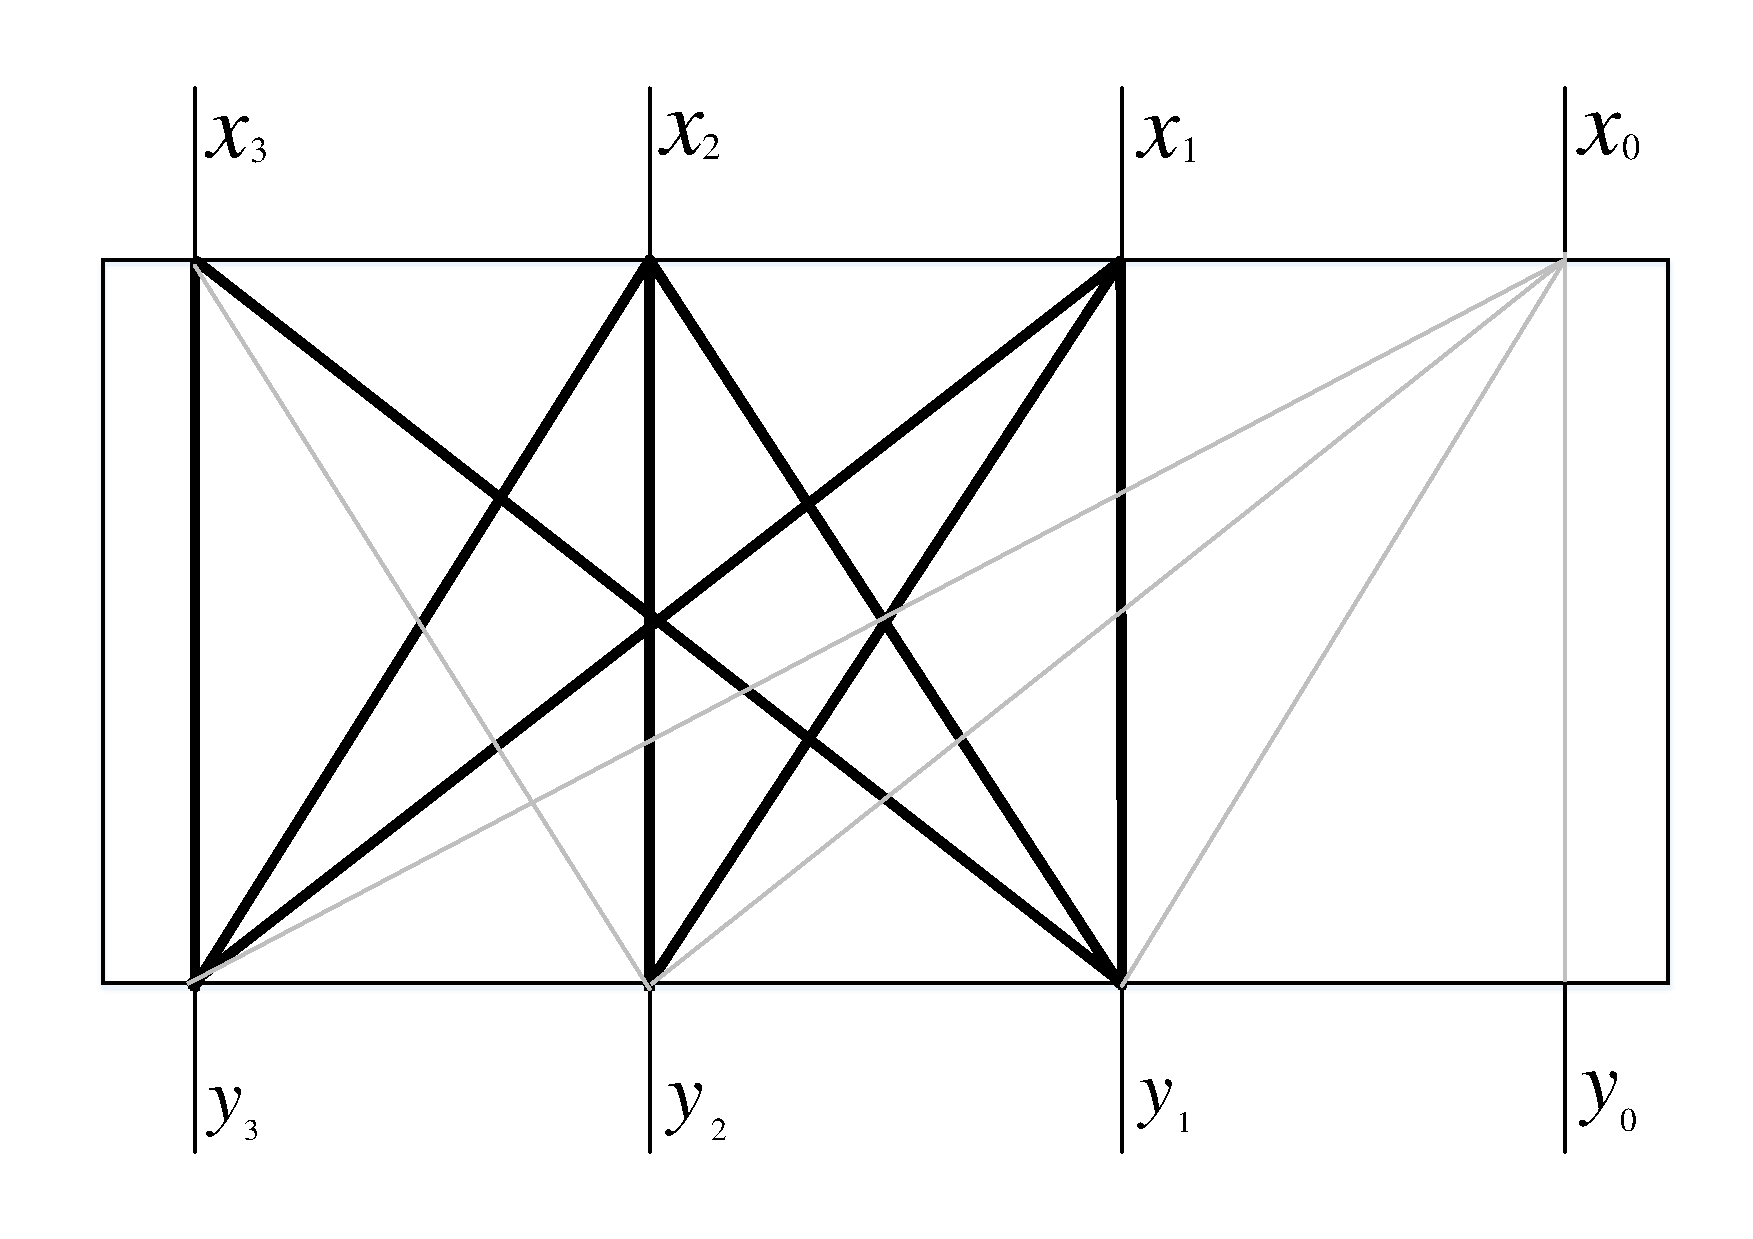
\includegraphics[width=0.9\textwidth,height = 6cm]{images/S-box_PRESENT}
    \caption{1 bit trails in the S-box of PRESENT.}
    \label{fig:S-box}
\end{figure}


\begin{figure}[h!]
    \centering
    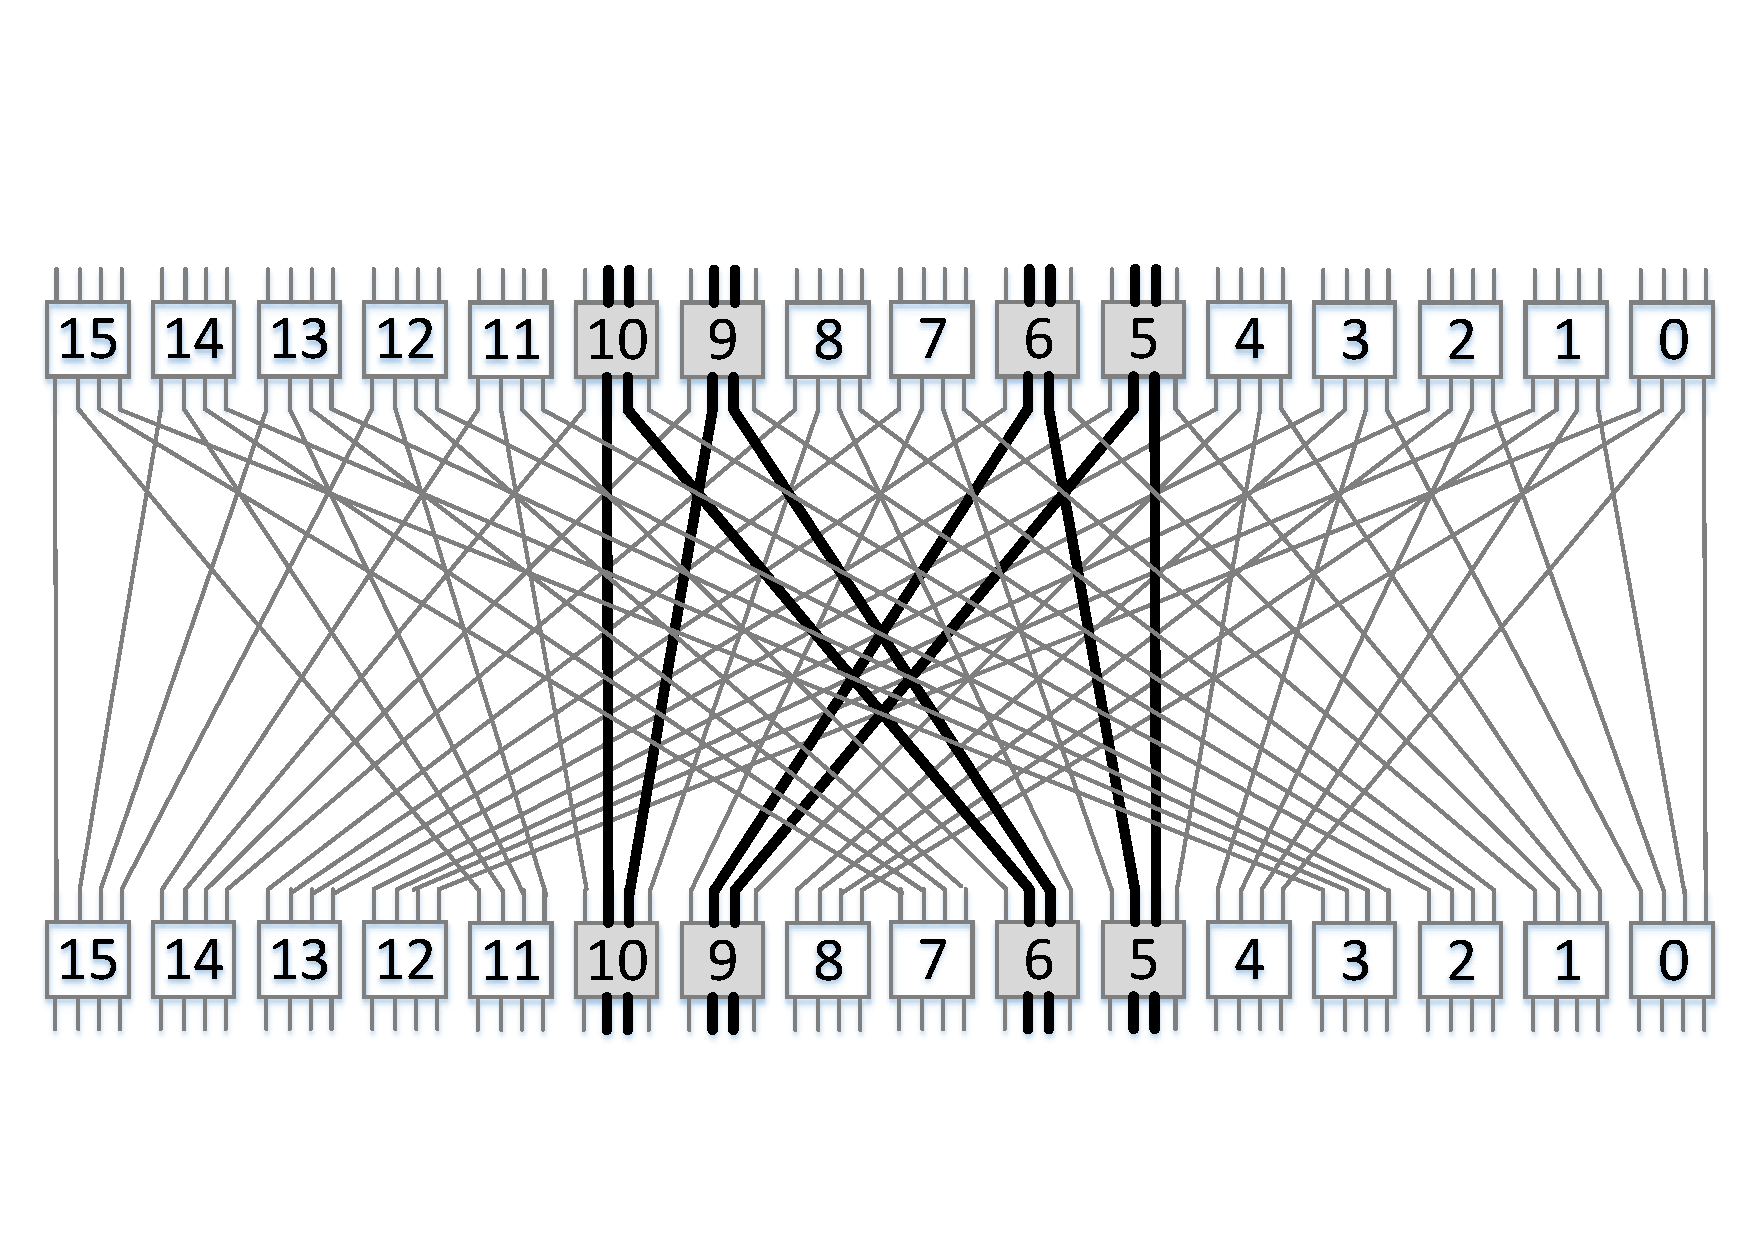
\includegraphics[width=0.9\textwidth]{images/presentCipherPoorDiffusionweakness}
    \caption{Weakness in PRESENT \cite{SSA_Collard_Standaert}.}
    \label{fig:present_weakness}
\end{figure}
There is a weakness in the permutation layer of PRESENT as described in Figure \ref{fig:present_weakness} \cite{SSA_Collard_Standaert}. The size of a block is $n=64$. Counting the plaintext bits starting from $0$ from the right, the $21,22,25,26,37,38,41,42$ bits are active only in $4$ S-boxes. And none of these bits are $x_0,x_3$ or $y_2$. So, it is expected that if we fix these $8$ bits (extreme non-uniformity) for each plaintext that we encrypt, then after encrypting sufficiently large amount of plaintexts, the ciphertexts will also have non-uniformity in the same $8$ bits. That is, the evolution of these $8$ bits are not random enough. As a result, we have a partitioning of the plaintext and ciphertext space. In the partitioning $s = q = 8$, $t = r = 56$, $B_s = B_q = \left\lbrace 21,22,25,26,37,38,41,42 \right\rbrace$ and $B_t = B_r = \left\lbrace 0,1,...,63  \right\rbrace \setminus B_s$.
\par \noindent Another interesting SS trail is mentioned in Figure \ref{fig:27bittrailPRESENT}. This trail has $27$ bits at its input and $27$ bits at its output. There are $9$ active S-boxes. Every S-box has $3$ input and $3$ output bits. That means in every S-box there are $3 \times 3 = 9$ different $1$ bit to $1$ bit trail. Note that this SS trail includes $x_3,y_2$ simultaneously which is unlike the principle we discussed in previous section. The reason, it is still a good SS trail is, out of the $9$ trails in every S-box, $x_3,y_2$ bits are involved in only one of them simultaneously. This results into $8$ active trails in every S-box whereas by excluding both of them we could have at most $2 \times 2 = 4$ active trails in every S-box. That means, even though $x_3,y_2$ has zero correlation among them across the S-box, it is still useful to include them in a trail as they contribute in generating other active trails.
\begin{figure}[h!]
    \centering
    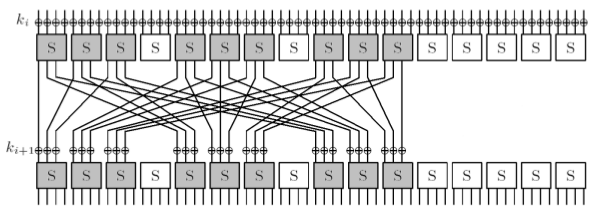
\includegraphics[width=0.9\textwidth]{images/27bittrailPRESENT}
    \caption{Weakness in PRESENT \cite{SSA_Collard_Standaert}.}
    \label{fig:27bittrailPRESENT}
\end{figure}

\section{Exploiting the Weakness}
In \cite{SSA_Collard_Standaert}, the authors proposed two techniques to exploit the weakness. In both of the techniques a sufficient number of chosen plaintexts are encrypted where $x_s$ part of $x$ is fixed to a value $a$.

\subsection{Comparing with Model Distribution} In order to exploit this weakness, the model distribution of $y_q$ part of $y$ is evaluated by Algorithm \ref{alg:theoretical_distribution} for each key guess. For one key guess at each round, the work needed to compute the model distribution of the target trail after $r$ round is equivalent to $r \cdot 2^{16}$ partial encryptions. Once the model distributions are computed, the key of the model distribution that minimizes the distance with the distribution computed from a secret key is accepted to be the correct key. 
\begin{algorithm}
\caption{: Computing model distribution}
\label{alg:theoretical_distribution}
\begin{algorithmic}[1]
\State Input: $8$-bit subkey guess $sk$ and the $8$-bit input distribution $distrib\_in[256]$
\State Output: the $8$-bit output distribution $distrib\_out[256]$\\
\State initialize $distrib\_out[256]$ to the all-zero state
\For {$8$-bit values $text$}
	\For {$8$-bit values $rand$}
		\State fix the $8$-bit trail to $text$ and xor with $sk$
		\State fix the $8$-bit non-trail to $rand$
		\State apply the S-boxes
		\State apply the permutation
		\State evaluate the value of the $8$ bit trail out
		\State update $distrib\_out[out]= distrib\_out[out] + distrib\_in[text]/256$;
	\EndFor
\EndFor
\end{algorithmic}
\end{algorithm}
\par \noindent To verify the practicability of the attack model, Collard and Standaert have conducted an experiment on reduced-round version of PRESENT. To reduce the number of key guess, they have simplified the key scheduling algorithm by using the same key in each round. They have used $2^{30}$ chosen plaintexts. In all those plaintexts, the $8$ bits (mentioned in Figure \ref{fig:present_weakness} in bold lines) are fixed, and the other $56$ bits are varied. All those plaintexts are encrypted where round keys are kept fixed in each round. Then they have computed the distribution of those fixed $8$ bits at the end of $2,4,6$ and $8$ round. These experimental distributions computed from the real cipher itself with reduced-round and modified key scheduling algorithm is compared with the model distributions computed from Algorithm \ref{alg:theoretical_distribution} for $2,4,6$ and $8$ rounds. According to this simplified experiment, both experimental and model distributions present a significant deviation from uniform as expected. \par \noindent They also have made an observation on the distance in between the experimental and model distributions. First they have computed the experimental and model distributions of the concerned $8$ bits at the end of $2,4,6$ and $8$ rounds for the key byte $32$ (i.e. $00100000$). Then they have computed the model distributions of these $8$ bits for all possible $256$ sub-keys at the end of $2,4,6$ and $8$ rounds. Finally they have plotted the distance in between the model distribution for every possible key bytes and model disribution of key byte $32$. For the sake of discussion, let us call this distance to be model-model distance. They also have plotted the distance in between the model distribution for every possible key bytes and experimental disribution of key byte $32$. Let us call this distance to be model-experiment distance. It has been found that the distance between the model-model and model-experiment distance is minimized at the correct key. This indicates that the model distribution captures the essence of the experimental distribution. \par \noindent In both of the experiments it has been found that the deviation tends to decrease with number of rounds. So, as the number of rounds increases, to find significant deviation, the number of chosen plaintext is also needed to be increased. In other words, as the number of rounds increases, the data complexity of the attack also increases.
\par \noindent However, in the attack mentioned above, the effect of the key scheduling algorithm has been ignored to show that the basic idea works in principle. Now considering the key scheduling algorithm, demands more key bits to be guessed as the round key changes in every round. As for one round we need to guess at most $8$ bits, we are in need of guessing at most $r \times 8$ bits after $r$ rounds. According to Collard and Standaert, for $12$ rounds of PRESENT, $63$ key bits have to be guessed, meaning, there are $2^{63}$ different possible keys in effect. For each key guess, after $r$ rounds, we are in need of computing $r \times 2^{16}$ partial encryptions. Which implies that we are in need of $2^{63} \times r \times 2^{16}$ partial encryptions. We see that the attack becomes quite impossible even with $12$ rounds because of its time complexity. In the next section, we present a tricky way to overcome this problem. The idea is the same as in commonly used statistical linear and differential attacks. Instead of guessing key bits on the intermediate rounds, make a prediction about the behaviour of the cipher over those rounds that holds on the average over the keys.

\subsection{Distinguishing Attack:} Computing the theoretical distribution is costly. To overcome this problem, they suggest a distinguishing attack which we will explain in brief here. The plaintexts are encrypted using $r$-rounds of PRESENT and record the distribution of the ciphertexts for the $16$ bits at the output of the $4$ active $S$-box in the last round. Given this experimental distribution, it is possible to compute the output distribution of the target $8$-bit trail one round before by a classical partial decryption process. For one key guess, the evaluation of such $r-1$-round distribution requires $2^{16}$ computations. For the corect key guess, the experimental $8$-bit distribution in the $r-1$-round is expected to be more non-uniform than for any other guess. This is because decrypting with a wrong guess is expected to have the same effect as encrypting one more round. Thus it is expected to distinguish the correct key from the wrong ones by computing the distance between a partially decrypted distribution and the uniform distribution. If the attack works properly, the distribution with the highest distance should correspond to the correct key. \par \noindent There are extensions of this distinguishing attack. The same attack can be made by increasing the number of fixed plaintext bits or by using multiple fixations of the fixed bits or by doing partial decryption for $2$ rounds instead of $1$ round. However, all these extensions require to distinguish a distribution from uniform distribution. The statistical model developed in this work is a statistic $T$ which can be used to perform a statistical test that can distinguish the computed distribution in between two known distributions. In the next sections, we have defined formally the notion of a distribution. We will also recall some known distributions and their properties as they will be useful in finding the statistical model. In the next chapter we have presented how to perform a statistical test to distinguish a distribution between two given distributions. In the next chapter we have defined the statistic $T$ and used it to develop a SS distinguisher in Chapter \ref{chapter:statistical_distinguishers}. In Chapter \ref{chapter:data_complexity_of_SSA}, we have shown how the success probability of the statistical test is related with the number of plaintexts we encrypt before performing the statistical test.